\documentclass{standalone}

\usepackage{verbatim}
\usepackage{pst-circ}

\usepackage{pgfplots}
\usepgfplotslibrary{polar}
\pgfplotsset{compat=1.10}

\pgfplotsset{mypolarplot/.style={%
  clip=false, 
  domain=0:360,
  samples=180,
  grid=both, 
  major grid style={black}, 
  minor x tick num=3,
  minor y tick num=1,
  xtick={0,45,...,359},
  xticklabels={%
    $0$,
    $\frac{ \pi}{4}$,
    $\frac{ \pi}{2}$,
    $\frac{3\pi}{4}$,
    $\pi$,
    $\frac{5\pi}{4}$,
    $\frac{3\pi}{2}$,
    $\frac{7\pi}{4}$
  },
  yticklabel style={anchor=north}, 
}}

\begin{document}
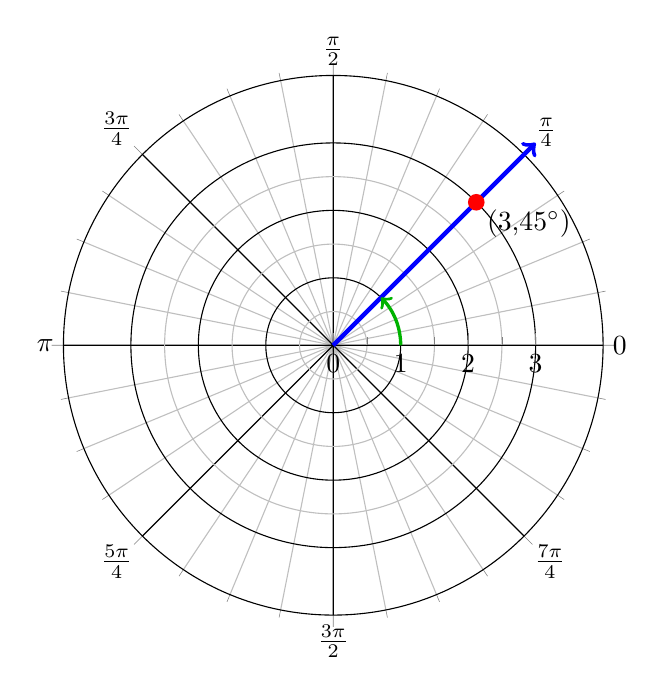
\begin{tikzpicture}
\begin{polaraxis}[%
  ymax=4,
  ytick={0,1,2,3},
  mypolarplot,
]


\draw [ultra thick, blue,  -> ] (0, 0) -- (300, 300 ) ;
\fill [red] (212, 212) circle (3 pt) ;

\draw (290, 180) node {(3,$45^\circ $) } ;
\draw [ very thick, -> , green!70!black ] (100, 0) arc (0:45:100);

\end{polaraxis}
\end{tikzpicture}
\end{document}